%%%%%%%%%%%%%%%%%%%%%%%%%%%%%%%%%%%%%%%%%
% Beamer Presentation
% LaTeX Template
% Version 1.0 (10/11/12)
%
% This template has been downloaded from:
% http://www.LaTeXTemplates.com
%
% License:
% CC BY-NC-SA 3.0 (http://creativecommons.org/licenses/by-nc-sa/3.0/)
%
%%%%%%%%%%%%%%%%%%%%%%%%%%%%%%%%%%%%%%%%%

%----------------------------------------------------------------------------------------
%	PACKAGES AND THEMES
%----------------------------------------------------------------------------------------

\documentclass[t]{beamer}

\mode<presentation> {

% The Beamer class comes with a number of default slide themes
% which change the colors and layouts of slides. Below this is a list
% of all the themes, uncomment each in turn to see what they look like.

%\usetheme{default}
%\usetheme{AnnArbor}
%\usetheme{Antibes}
%\usetheme{Bergen}
%\usetheme{Berkeley}
%\usetheme{Berlin}
%\usetheme{Boadilla}
%\usetheme{CambridgeUS}
%\usetheme{Copenhagen}
%\usetheme{Darmstadt}
%\usetheme{Dresden}
%\usetheme{Frankfurt}
%\usetheme{Goettingen}
%\usetheme{Hannover}
%\usetheme{Ilmenau}
%\usetheme{JuanLesPins}
%\usetheme{Luebeck}
\usetheme{Madrid}
%\usetheme{Malmoe}
%\usetheme{Marburg}
%\usetheme{Montpellier}
%\usetheme{PaloAlto}
%\usetheme{Pittsburgh}
%\usetheme{Rochester}
%\usetheme{Singapore}
%\usetheme{Szeged}
%\usetheme{Warsaw}

% As well as themes, the Beamer class has a number of color themes
% for any slide theme. Uncomment each of these in turn to see how it
% changes the colors of your current slide theme.

%\usecolortheme{albatross}
%\usecolortheme{beaver}
%\usecolortheme{beetle}
%\usecolortheme{crane}
%\usecolortheme{dolphin}
%\usecolortheme{dove}
%\usecolortheme{fly}
%\usecolortheme{lily}
%\usecolortheme{orchid}
%\usecolortheme{rose}
%\usecolortheme{seagull}
%\usecolortheme{seahorse}
%\usecolortheme{whale}
%\usecolortheme{wolverine}

%\setbeamertemplate{footline} % To remove the footer line in all slides uncomment this line
%\setbeamertemplate{footline}[page number] % To replace the footer line in all slides with a simple slide count uncomment this line

\setbeamertemplate{navigation symbols}{} % To remove the navigation symbols from the bottom of all slides uncomment this line
}

\usepackage{graphicx} % Allows including images
\usepackage{booktabs} % Allows the use of \toprule, \midrule and \bottomrule in tables
\usepackage{fancyvrb} % Tabs in verbatim
\usepackage{ulem} % Strikeout
%----------------------------------------------------------------------------------------
%	TITLE PAGE
%----------------------------------------------------------------------------------------

\title[FPGA102]{FPGA102: More FPGA} % The short title appears at the bottom of every slide, the full title is only on the title page

\author{Josh Johnson} % Your name
\institute[] % Your institution as it will appear on the bottom of every slide, may be shorthand to save space
{ \\ % Your institution for the title page
\medskip
\textit{} % Your email address
}
\date{28/10/2019} % Date, can be changed to a custom date

\begin{document}

\begin{frame}
\titlepage % Print the title page as the first slide
\end{frame}

%----------------------------------------------------------------------------------------
%	PRESENTATION SLIDES
%----------------------------------------------------------------------------------------

\begin{frame}
\frametitle{Overview}
\begin{itemize}
\item Schematic / PCB Design
\item Silicon Level
\item Toolchain
\item Demo time
\begin{itemize}
	\item PWM x 3
	\item UART TX, RX
	\item Dot
\end{itemize}

\end{itemize}
\vspace{20mm}
Project Files: \url{github.com/joshajohnson/CBRhardware}\\
Also on the memory stick being passed around
\end{frame}

%----------------------------------------------------------------------------------------

\begin{frame}[t]
\frametitle{Schematic / PCB Design}
\begin{figure}
	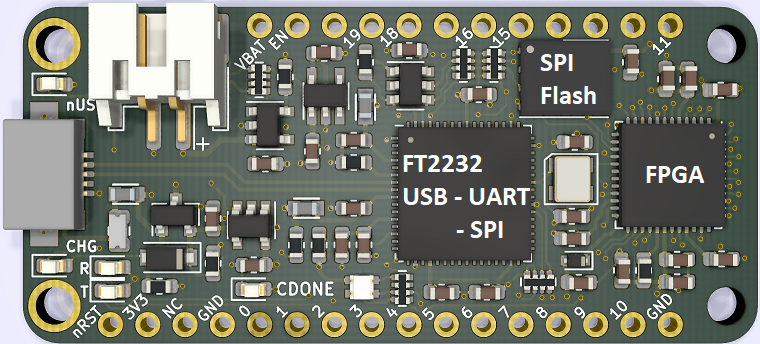
\includegraphics[width=\linewidth]{top_render_annotated.png}
\end{figure}
\end{frame}

%----------------------------------------------------------------------------------------

\begin{frame}[t]
	\frametitle{Silicon Level}
	Following slides stolen from Dave Shah
	\begin{figure}
		\includegraphics[width=\linewidth, page=1]{oshug.pdf}
	\end{figure}
\end{frame}

%----------------------------------------------------------------------------------------

\begin{frame}[t]
	\frametitle{Silicon Level}
	\begin{figure}
		\includegraphics[width=\linewidth, page=2]{oshug.pdf}
	\end{figure}
\end{frame}

%----------------------------------------------------------------------------------------

\begin{frame}[t]
	\frametitle{Silicon Level}
	\begin{figure}
		\includegraphics[width=\linewidth, page=4]{oshug.pdf}
	\end{figure}
\end{frame}

%----------------------------------------------------------------------------------------

\begin{frame}[t]
	\frametitle{Silicon Level}
	\begin{figure}
		\includegraphics[width=\linewidth, page=5]{oshug.pdf}
	\end{figure}
\end{frame}

%----------------------------------------------------------------------------------------

\begin{frame}[t]
	\frametitle{Silicon Level}
	\begin{figure}
		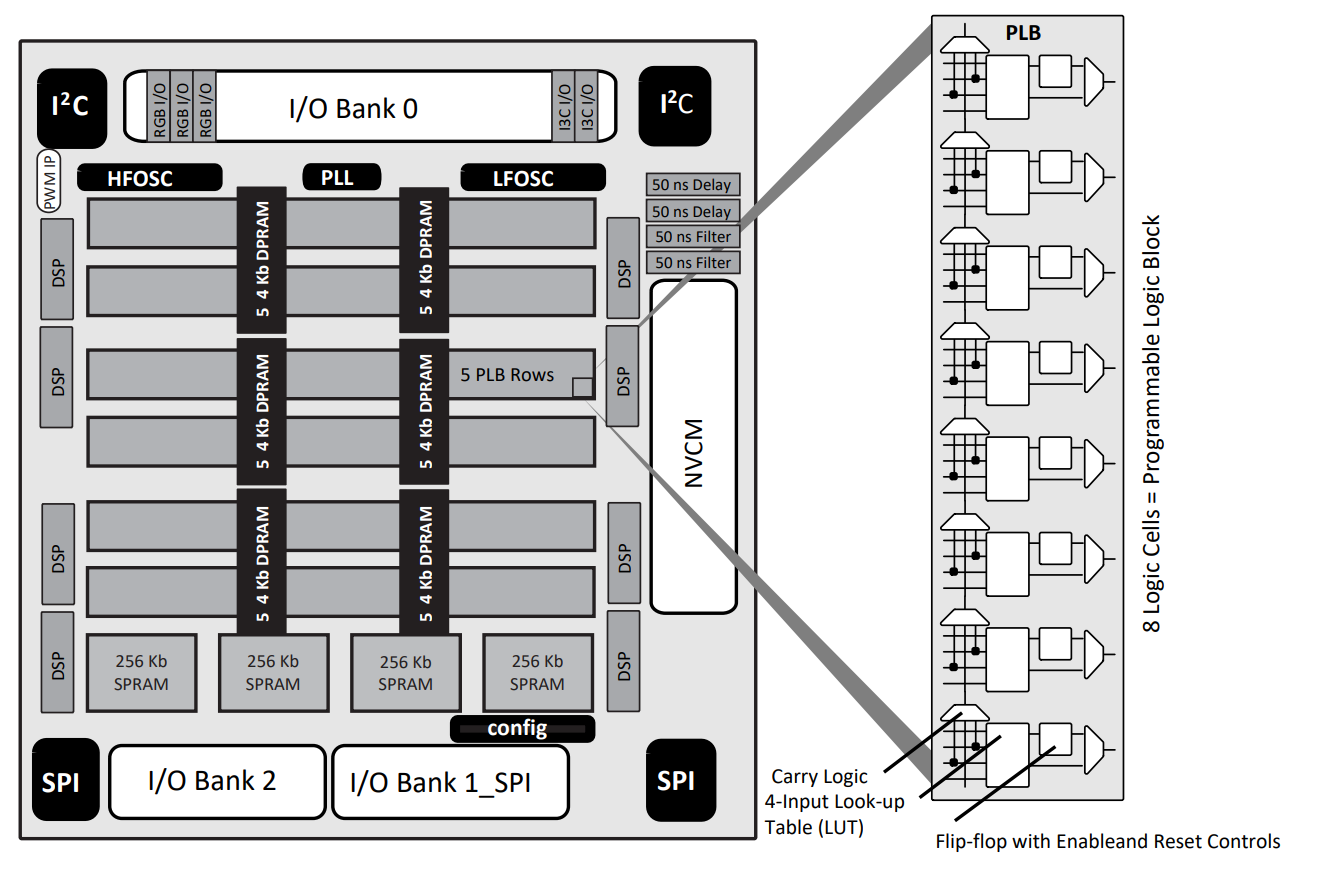
\includegraphics[width=0.9\linewidth]{ice40-internals.png}
	\end{figure}
\end{frame}

%----------------------------------------------------------------------------------------

\begin{frame}[t]
	\frametitle{Silicon Level}
	\begin{figure}
		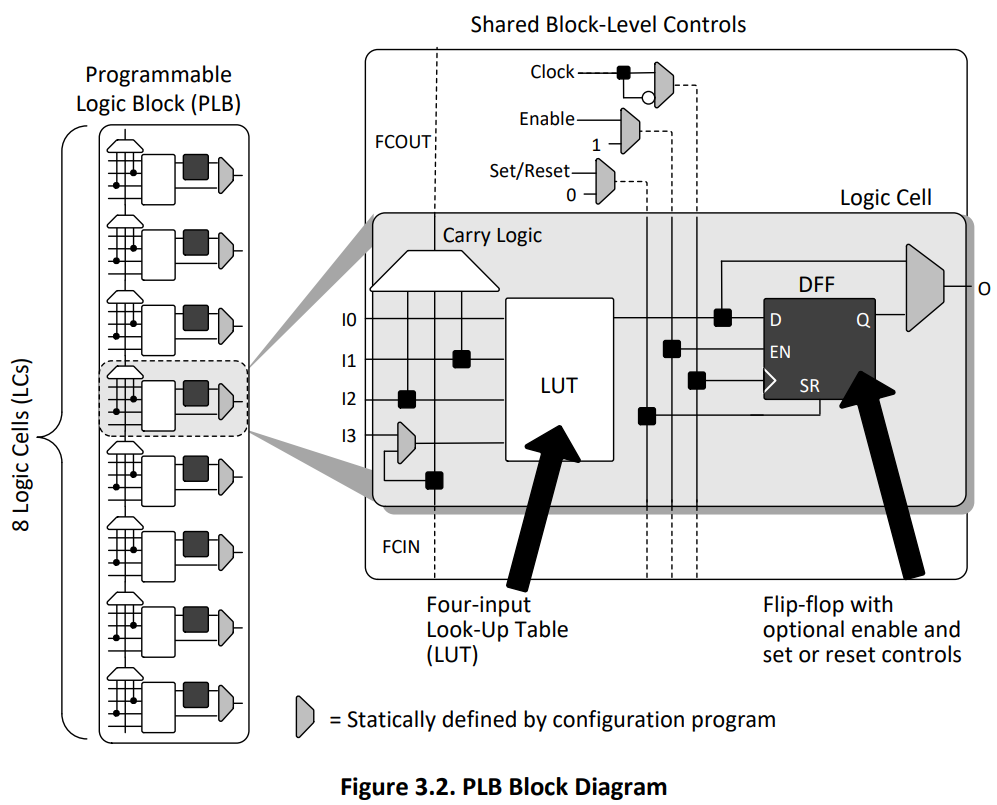
\includegraphics[width=0.8\linewidth]{plb-internals.png}
	\end{figure}
\end{frame}

%----------------------------------------------------------------------------------------

\begin{frame}[t]
	\frametitle{Silicon Level}
	\begin{figure}
		\includegraphics[width=\linewidth, page=8]{oshug.pdf}
	\end{figure}
\end{frame}

%----------------------------------------------------------------------------------------

\begin{frame}[t]
	\frametitle{Silicon Level}
	\begin{figure}
		\includegraphics[width=\linewidth, page=9]{oshug.pdf}
	\end{figure}
\end{frame}

%----------------------------------------------------------------------------------------

\begin{frame}[t]
	\frametitle{Toolchain}
	Steps required to turn Verilog into working hardware.
	\begin{itemize}
		\item Synthesis: Verilog to logic gates (Yosys)
		\item Place and Route: Physically connect LUTs in FPGA (nextPNR)
		\item Programming: Load bitstream onto FPGA (iceStorm)
	\end{itemize}
	Watch this for more info: https://www.youtube.com/watch?v=A5AHglpfdtQ
\end{frame}

%----------------------------------------------------------------------------------------

\begin{frame}[t]
	\frametitle{Synthesis}
	\begin{figure}
		\includegraphics[width=\linewidth, page=14]{oshug.pdf}
	\end{figure}
\end{frame}
%----------------------------------------------------------------------------------------

\begin{frame}[t]
	\frametitle{Place and Route}
	\begin{figure}
		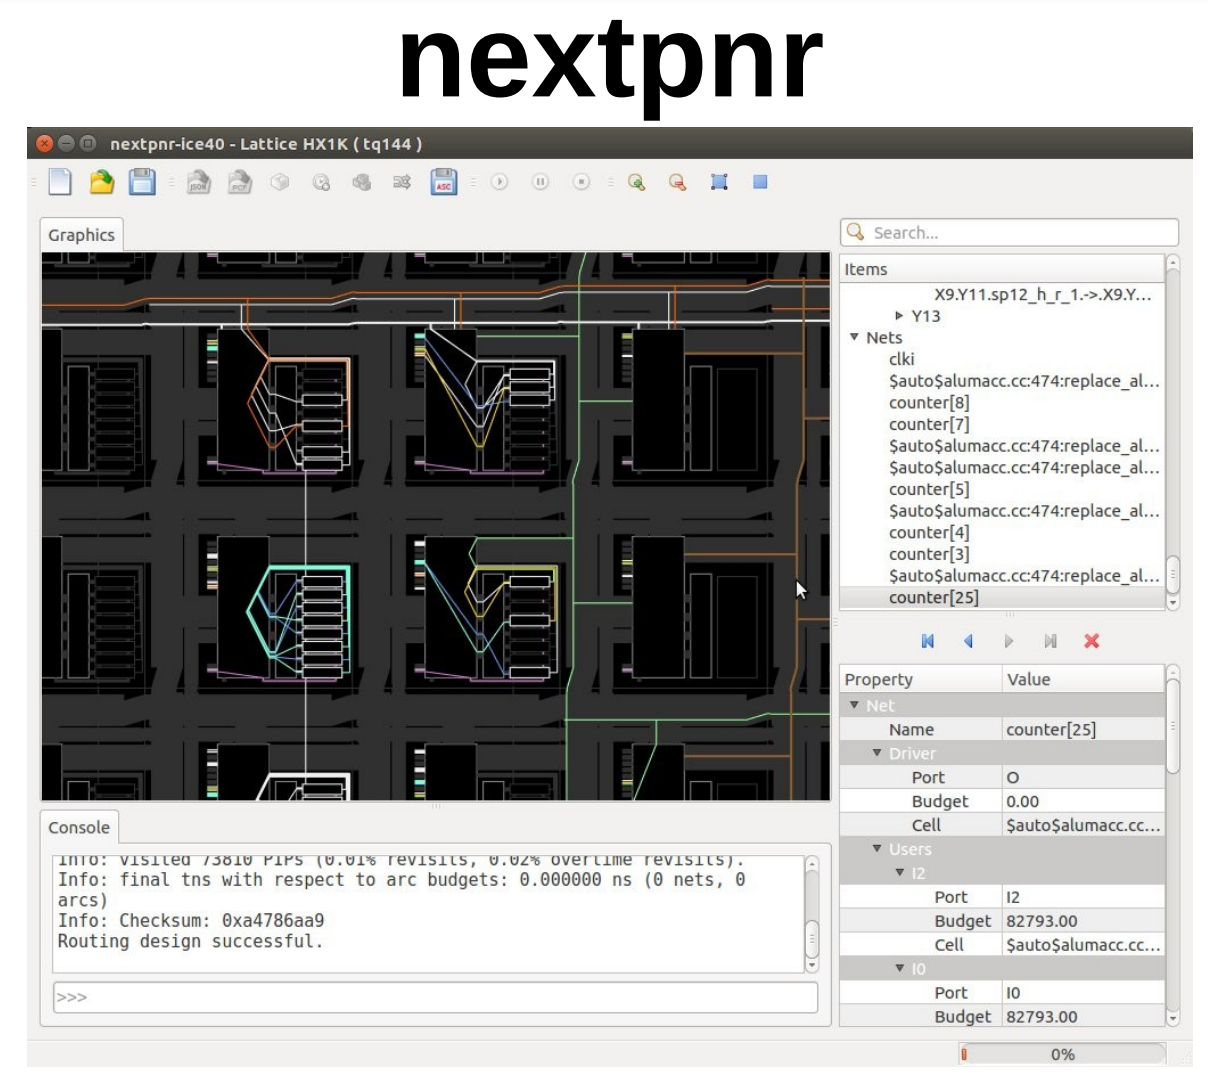
\includegraphics[width=0.7\linewidth]{nextpnr.png}
	\end{figure}
\end{frame}

%----------------------------------------------------------------------------------------

\begin{frame}[t]
	\frametitle{Demo Time - PWM}
	Three Demos showing how to PWM a LED
	\begin{itemize}
		\item Basic linear fade up / down
		\item Above but with three bugs - how to debug / setup simulation
		\item Gamma corrected PWM
	\end{itemize}
\end{frame}

%----------------------------------------------------------------------------------------

\begin{frame}[t]
	\frametitle{Simulation Setup}
	\begin{itemize}
		\item Install GTKwave and Icarus Verilog
		\item Create \texttt{fileName\_tb.v} test bench and add required code
		\item Alternatively, can run \texttt{make new NAME="newName"} to copy from blink example with all files names changed
		\item Run \texttt{make simulate} to simulate and view waveforms
		\item Upon setting up GTKwave, go \texttt{file->write save file} to save current display
		\item Wayne has documented the process (see resources)
		\item Easier if I just show you...
	\end{itemize}
\end{frame}

%----------------------------------------------------------------------------------------

\begin{frame}[t]
	\frametitle{LED Matrix}
	\begin{figure}
		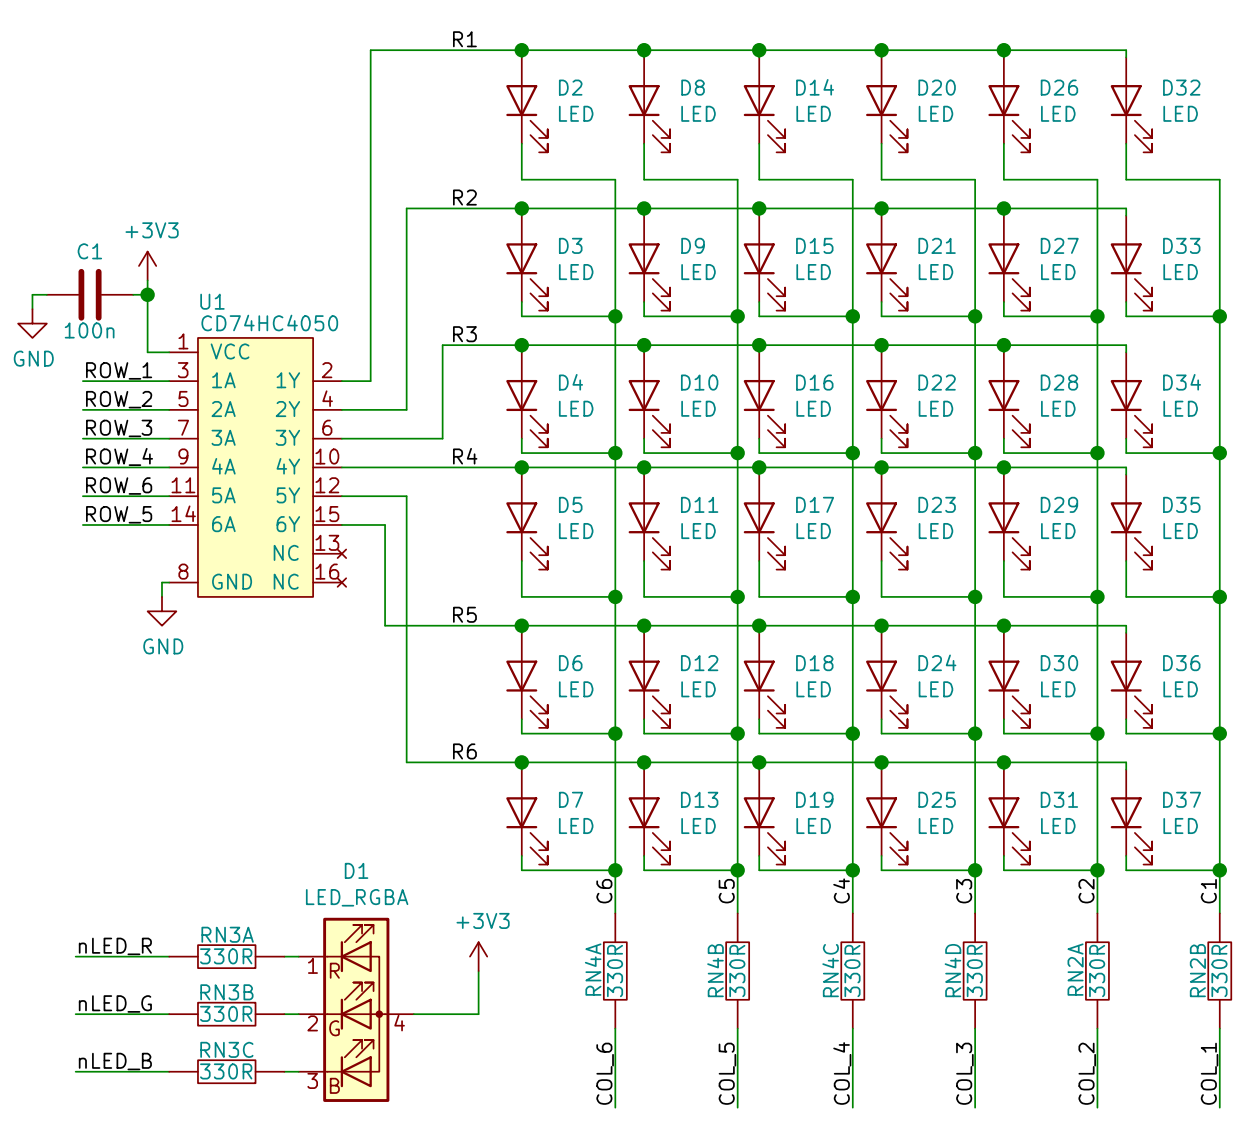
\includegraphics[width=0.6\linewidth]{ledMatrix.png}
	\end{figure}
	Yes (0,0) is top right corner (there is a reason for this!)
\end{frame}

%----------------------------------------------------------------------------------------

\begin{frame}[t]
	\frametitle{UART}
	Standard UART frame: 9600 Baud, 1 start bit (low), 8 data bits, LSB first, 1 stop bit (high).\\
	To transmit: set pin as required. \\
	To receive: sample half way through bit period
	\begin{figure}
		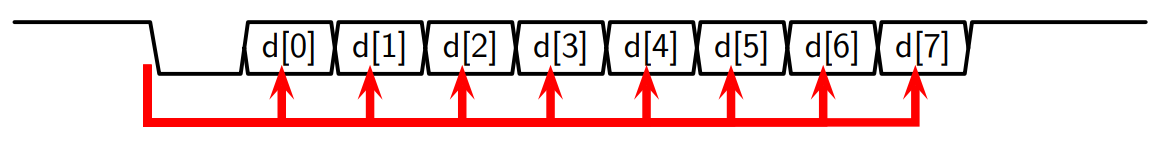
\includegraphics[width=\linewidth]{uart.png}
	\end{figure}
	Image stolen from ZipCPU
\end{frame}

%----------------------------------------------------------------------------------------

\begin{frame}
\frametitle{The End}
Links to resources: \texttt{fpga102/README.md}
\vspace{5mm}

\textbf{Next month (11/11/19)}\\
Unprepared talk on Electronic Test and Measurement, highlighting what tool is right for the job, limitations of equipment, along with how to do things on the cheap, and an overview of the VNA I built.\\[5pt]

\textbf{Future Months}\\
I won't be here - talk to Silvio if you want to run the meetup


\vspace{10mm}
Say Hello! \\
BSidesCbr Slack: josh\\
Twitter:  @\textunderscore joshajohnson\\
Email: josh@joshajohnson.com\\
\vspace{4mm}

Project Files: \url{github.com/joshajohnson/CBRhardware}\\
\end{frame}


\end{document} 